\documentclass[SE,lsstdraft,authoryear,toc]{lsstdoc}
\input{meta}

% Package imports go here.
\usepackage{xcolor}
\usepackage{graphicx} % Formats for images
\usepackage{booktabs} % For \toprule, \midrule and \bottomrule
\usepackage{multirow} % Required for multirows
\usepackage{pdflscape}
\usepackage{subcaption}
\usepackage{tikz}
\usepackage{pgfplots}
\usepackage{booktabs}
\usepackage{caption}
% Local commands go here.

%If you want glossaries
%\input{aglossary.tex}
%\makeglossaries

\title{CCW/Rotator Synchronous Motion Limit Switch Characterization with ComCam}

% Optional subtitle
% \setDocSubtitle{A subtitle}

\author{%
Austin Roberts, Holger Drass, Brian Stalder
}

\setDocRef{SITCOMTN-053}
\setDocUpstreamLocation{\url{https://github.com/lsst-sitcom/sitcomtn-053}}

\date{\vcsDate}

% Optional: name of the document's curator
% \setDocCurator{The Curator of this Document}

\setDocAbstract{%
The Camera Cable Wrap / Camera Rotator synchronous motion limit switch characterization will identify the optimal placement of the limit switches based on a variety of factors. This is the follow on work required by \href{https://sitcomtn-011.lsst.io/}{SITCOMTN-011} due to the design differences between the originally design bulkhead plate and the redesigned bulkhead plate which houses the limit switches and the addition of a representative load on the Rotator.
}

% Change history defined here.
% Order: oldest first.
% Fields: VERSION, DATE, DESCRIPTION, OWNER NAME.
% See LPM-51 for version number policy.
\setDocChangeRecord{%
  \addtohist{1}{YYYY-MM-DD}{Unreleased.}{Austin Roberts}
}


\begin{document}

% Create the title page.
\maketitle
% Frequently for a technote we do not want a title page  uncomment this to remove the title page and changelog.
% use \mkshorttitle to remove the extra pages

% ADD CONTENT HERE
% You can also use the \input command to include several content files.
\section{Executive Summary}

This characterization activity covers the follow-on work identified in the previous characterization activity as defined in \href{https://sitcomtn-011.lsst.io/}{SITCOMTN-011}. The characterization of the limit switches that protect the utility lines that run from the Camera Cable Wrap to the back of the Camera was performed on the Tekniker designed bulkhead plate which connects to the Camera Cable Wrap. This characterization was performed on the Camera Cart on the 3rd floor of the observatory without ComCam or LSSTCam installed on the Camera Rotator. The primary goal of the characterization was to determine the optimal placement of the limit switches. Prior to completing the characterization it was brought to our attention that the bulkhead plate had been redesigned by SLAC due to complexities with the camera installation. The previous characterization determined that the limit switches should be placed at \textbf{+/- 3.5 deg} from the center line. Due to differences in the design of the SLAC bulkhead plate and this characterization being performed without a representative load and CG on the Rotator, it was determined that this characterization will need to be performed again on the SLAC bulkhead plate after ComCam is installed on the Rotator and before the utilities are connected.
The characterization has been performed with the new configuration which now includes the SLAC designed bulkhead plate and ComCam installed on the Camera Rotator.
{\color{red}
\textbf{TBD}}


\section{Overview}

\subsection{System Overview}
The system being characterized is the Camera Cable Wrap (CCW), the Camera Rotator, and the Wobble Assembly. The Wobble assembly connects to the CCW via the bulkhead plate and to the ComCam/LSSTCam via the wobble plate per LTS-156. The bulkhead plate has a limit switch mounted in the positive and negative direction in relation to the 0 degree location and a joint with adjustable detection cams in the positive and negative direction. These features are designed to protect the utility lines from damage due to excessive twist between the CCW and the Camera. See Figure \ref{fig:Figure_1} below. The bulkhead plate and the limit switches rotate with the CCW and the wobble plate, linkage rods, and the detection cams rotate with the Camera. The Camera is rotated by the Camera Rotator. Activating either the positive or negative limit switch will generate a Safe Torque Off (STO) to the CCW Interlock System and the Rotator Interlock System to remove power to the drives. The characterization was performed on the Camera Cart on the 3\textsuperscript{rd} floor of the observatory.

\begin{figure}[h!]
  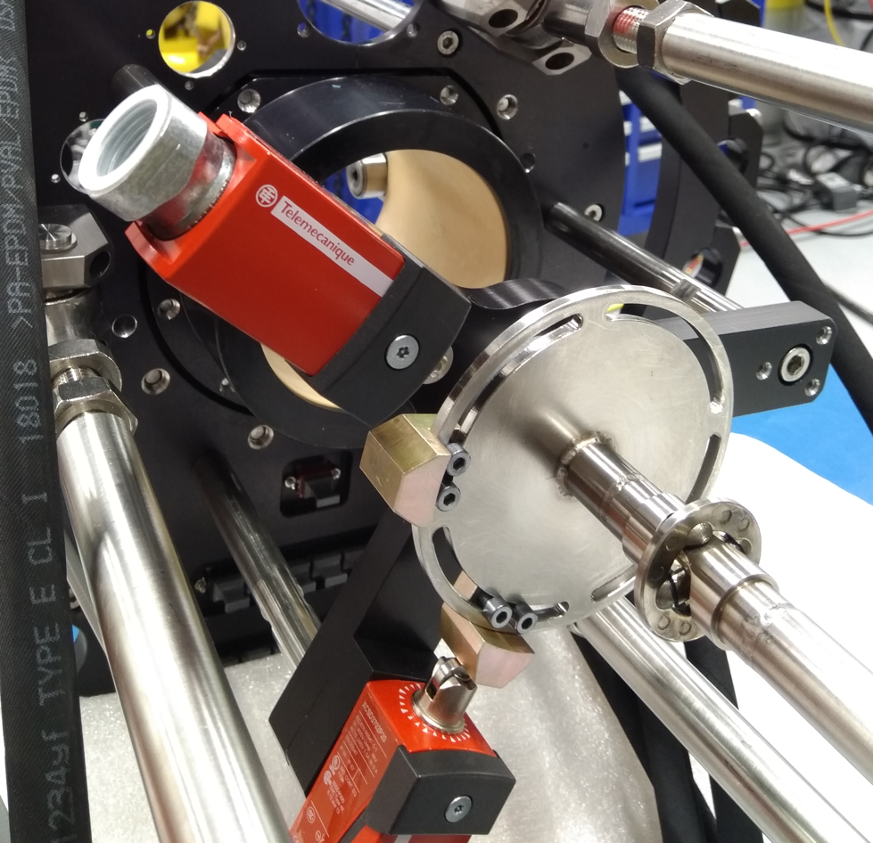
\includegraphics[width=\linewidth]{media/Figure_1.png}
  \caption{Bulkhead Plate with Limit Switches}
  \label{fig:Figure_1}
\end{figure}

\subsection{Objective}

The objective of this characterization is to find the allowable position
range of the positive and negative limit switches and provide a
recommendation of where they should be positioned. This requires finding
the exact position that the limit switches are currently activated,
finding the back off distance required to release the limit switches,
and finding the maximum distance for the CCW and Camera Rotator to come
to a complete stop after activating the limit switches.

\subsection{Requirements}

The following are the relevant requirements for the synchronous motion
between the CCW and the Camera Rotator.

\underline{LTS-103}

\begin{itemize}
\item
  3.10.13 MCS Camera Cable Wrap Positioning Command

  \begin{itemize}
  \item
    \textbf{Specification:} The camera cable wrap shall be slaved to the
    camera rotator.
  \end{itemize}
\end{itemize}

\underline{LTS-218}

\begin{itemize}
\item
  3.3.7 Rotation Drive Synchronization with Camera Rotator

  \begin{itemize}
  \item
    \textbf{Specification:} During slewing and tracking, the camera
    cable wrap rotation shall remain synchronized with the camera
    rotator to better than 2.2 degrees. An absolute rotation sensing
    encoder shall be incorporated on the rotation drive unit to provide
    position feedback to the telescope control system (TCS).
  \end{itemize}
\item
  3.3.8.1 Slewing Velocity Range

  \begin{itemize}
  \item
    \textbf{Specification:} The rotation drive unit shall be able to
    reach any velocity between 0 and 3.5deg/sec with a goal of
    5.25deg/sec in both rotation directions.
  \end{itemize}
\item
  3.16 Safety Pull Cord

  \begin{itemize}
  \item
    \textbf{Specification}: The functionality of the safety pull-cord
    has been replaced by limit switches now specified in LTS-156.
  \end{itemize}
\item
  3.3.1 Rotation Range

  \begin{itemize}
  \item
    \textbf{Specification:} The camera cable wrap shall be designed to rotate
    over a 180 degree operational range (+/- 90 degrees either side of
    centered position). This 180 degree range must be achievable without
    exceeding any software limit, limit switch or hard stop,
    consequently, an additional 8 degrees (+/-4) is required to
    accommodate these items. The software limits shall limit the motion
    to the 180 degree range. The limit switches shall stop the motion
    within 2 degrees of meeting this maximum operational range. The hard
    stops shall stop the motion within another 2 degrees of the limit
    switches.
  \end{itemize}
\end{itemize}

\underline{LTS-156}

\begin{itemize}
\item
  The limits shall be adjusted to nominally stop rotation for any twist
  between the bulkhead plate and the wobble plate greater than +/- 3.5
  degrees with adjustment range from 2.5 degrees to 5 degrees.
\item
  The limit switch shall be tested over the range of travel of the
  wobble plate as specified below.

  \begin{itemize}
  \item
    The wobble plate radial motion is +/- 110mm.
  \item
    The wobble plate tilt about its center is +/- 3 degrees.
  \item
    The wobble plate Z motion is +/- 15mm.
  \end{itemize}
\end{itemize}

\underline{LTS-206}

\begin{itemize}
\item
  3.4.5.1 Rotator Slewing Velocity Range

  \begin{itemize}
  \item
    \textbf{Specification:} During a rotator slew, the Camera Rotator
    shall be able to reach any velocity between 0 and 3.5deg/sec with a
    goal of 5.25deg/sec in both rotation directions.
  \end{itemize}
\item
  3.4.4 Rotator Rotation Range

  \begin{itemize}
  \item
    \textbf{Specification:} The Camera Rotator shall be designed to
    rotate over a 180 degree operational range (+/-90 degrees TBR). This
    range must be achievable without reaching any software limit, limit
    switch or hard stop. The limit switches shall stop the motion within
    2 degrees of meeting this maximum operational range. The hard stops
    shall be within another 2 degrees of the limit switches.
  \end{itemize}
\end{itemize}

\underline{LSE-80}

\begin{itemize}
\item
  CA-TS-MEC-ICD-0058 Maximum Allowed Camera Motion at Bulkhead Plate

  \begin{itemize}
  \item
    \textbf{Specification:} The telescope shall ensure that the maximum
    transverse and axial motions of the back end of the camera utility
    trunk are no larger than \textbf{UTradialMotion} transverse,
    \textbf{UTaxialMotion} axial load, and \textbf{UTrotMotion} angular
    rotation around a radial line.
  \item
    UTrotMotion = 5 degrees
  \end{itemize}
\end{itemize}

\section{Characterization Tasks}\label{sec:Characterization Tasks}

The following sections define the tasks that were performed, the details of how they were performed, and the results of the task. Due to ComCam being installed, we will only be performing the characterization with the design velocities. We do not have any data showing what the emergency stopping maximum deceleration and jerk values are with a representative load on the camera rotator. We also do not have a transfer function for the forces from the camera rotator to ComCam. In order to avoid any issues due to these uncertainties we will perform the tasks using the camera rotator at 1 deg/s, then 2 deg/s, and finally the design velocity of 3.5 deg/s.

\subsection{Positive Limit Switch Activation Location}

To determine the exact location that the cam activates the positive
limit switch we moved the CCW slowly and in small increments to find
where the interlock was activated. We moved the CCW at a velocity of 0.1
deg/s and in 0.05 deg increments. This was only performed with the CCW
as it should not matter which system is used to activate the limit
switches at this low velocity and increments.

The positive limit switch was activated at \textbf{+2.81 deg}.

\subsection{Positive Limit Switch Release Location}

To determine where the positive limit switch is released, we first moved
the CCW slowly and in small increments to find where the interlock was
released. We moved the CCW at a velocity of 0.1 deg/s and in 0.05 deg
increments. This was only performed with the CCW because the CCW has the
override for the interlock and is defined to be the system used to
release the limit switch.

The positive limit switch was released at \textbf{+2.6 deg}.

Next, we moved at the design velocity of 3.5 deg/s in a single move in
the releasing direction to find where the limit switch is released which
is a real-world way that we would release the interlock. At these small
distances the velocity never reached the full design velocity. Each time
the limit switch was activated, we did a single move in the releasing
direction increasing by 0.05 deg until we found the location that the
limit switch was released.

The positive limit switch was released at \textbf{+2.65 deg}.

\subsection{Positive Limit Switch CCW Design Velocity Stopping Distance}

To determine the CCW stopping distance for the design velocity after
activating the positive limit switch we moved the CCW in the positive
direction with enough distance to reach a velocity of 3.5 deg/s before
activating the limit switch. This was repeated 5 times. To
calculate the stopping distance after activation we subtracted the
activation location determined in Section 3.1 from the position the CCW
came to a complete stop.

The maximum stopping distance after activating the positive limit switch
was found to be \textbf{0.47 deg}. See Appendix data for the data points
and Appendix efd for the EFD data.

\subsection{Positive Limit Switch Camera Rotator Design Velocity Stopping Distance}

To determine the Rotator stopping distance for the design velocity after
activating the positive limit switch we moved the Rotator in the
negative direction with enough distance to reach a velocity of 3.5 deg/s
before activating the limit switch. Since we defined the positive limit
switch to be the limit switch that is activated by the CCW moving in the
positive direction this correlates to the Rotator moving in the negative
direction. This was repeated 5 times. To calculate the stopping
distance after activation we subtracted the activation location
determined in Section 3.1 from the position the Rotator came to a
complete stop.

The maximum stopping distance after activating the positive limit switch
was found to be \textbf{0.69 deg}. See Appendix data for the data points
and Appendix efd for the EFD data.

\subsection{Negative Limit Switch Activation Location}

To determine the exact location that the cam activates the negative
limit switch we moved the CCW slowly and in small increments to find
where the interlock was activated. We moved the CCW at a velocity of 0.1
deg/s and in 0.05 deg increments.

The negative limit switch was activated at \textbf{-2.75 deg}.

\subsection{Negative Limit Switch Release Location}

To determine where the negative limit switch is released, we first moved
the CCW slowly and in small increments to find where the interlock was
released. We moved the CCW at a velocity of 0.1 deg/s and in 0.05 deg
increments. This was only performed with the CCW because the CCW has the
override for the interlock and is defined to be the system used to
release the limit switch.

The negative limit switch was released at \textbf{-2.45 deg}.

Next, we moved at the design velocity of 3.5 deg/s in a single move in
the releasing direction to find where the limit switch is released which
is a real-world way that we would release the interlock. At these small
distances the velocity never reached the full design velocity. Each time
the limit switch was activated, we did a single move in the releasing
direction increasing by 0.05 deg until we found the location that the
limit switch was released. This was repeated several times starting at
various distances from the limit switch when activating the limit switch
to see if the velocity to which the limit switch was activated
influences the distance required to release the limit switch.

The negative limit switch was released at \textbf{-2.5 deg}. We found
that the velocity at which the limit switch was activated did have an
effect on the releasing distance but it was not linear. We found that
there was a distance of approximately 3 deg from the limit switch where
the releasing distance required changed by 0.05 deg. We did not explore
this any further as it is not really relevant for this characterization
as we will take the maximum value.

\subsection{Negative Limit Switch CCW Design Velocity Stopping Distance}

To determine the CCW stopping distance for the design velocity after
activating the negative limit switch we moved the CCW in the negative
direction with enough distance to reach a velocity of 3.5 deg/s before
activating the limit switch. This was repeated 5 times. To
calculate the stopping distance after activation we subtracted the
activation location determined in Section 3.6 from the position the CCW
came to a complete stop.

The maximum stopping distance after activating the negative limit switch
was found to be \textbf{0.27 deg}. See Appendix data for the data points
and Appendix efd for the EFD data.

\subsection{Negative Limit Switch Camera Rotator Design Velocity Stopping Distance}

To determine the Rotator stopping distance for the design velocity after
activating the negative limit switch we moved the Rotator in the
positive direction with enough distance to reach a velocity of 3.5 deg/s
before activating the limit switch. Since we defined the negative limit
switch to be the limit switch that is activated by the CCW moving in the
negative direction this correlates to the Rotator moving in the positive
direction. This was repeated 5 times. To calculate the stopping
distance after activation we subtracted the activation location
determined in Section 3.6 from the position the Rotator came to a
complete stop.

The maximum stopping distance after activating the negative limit switch
was found to be \textbf{0.44 deg}. See Appendix data for the data points
and Appendix efd for the EFD data.

\begin{landscape}
\section{Recommendations}

\subsection{Characterization Results}

The tables below provides a summary of the calculations performed on the
data captured to determine the result of the tasks define in Section \ref{sec:Characterization Tasks}.

\begin{table}[h!]
  \begin{center}
    \caption{CCW Positive Limit Switch Characterization Calculation Results}
    \label{tab:table1}
    \begin{tabular}{r|c|r|c|r|c|c|c}
    \multicolumn{5}{l|}{\textbf{CCW Positive Limit Switch}} & Avg & Max & Std Dev\\
    \midrule
    Activation location: & 2.8 & & & & & & \\
    Release location: & 2.6 3.5 deg/s stopping location: & 3.246 & 3.27 & 0.0174356 \\
    Incremental delta: 0.2 3.5 deg/s stopping distance: & 0.446 & \textbf{0.47} & \\
    \end{tabular}
  \end{center}
\end{table}

\begin{table}[h!]
  \begin{center}
    \caption{CCW Negative Limit Switch Characterization Calculation Results}
    \label{tab:table2}
    \begin{tabular}{r|c|r|c|r|c|c|c}
    \multicolumn{5}{l|}{\textbf{CCW Negative Limit Switch}} & Avg & Max & Std Dev\\
    \midrule
    Activation location: & -2.75 & & & & & & \\
    Release location: & -2.45 3.5 deg/s stopping location: & -3.006 & -3.02 & 0.01019804 \\
    Incremental delta: 0.3 3.5 deg/s stopping distance: & 0.256 & \textbf{0.27} & \\
    \end{tabular}
  \end{center}
\end{table}

\begin{table}[h!]
  \begin{center}
    \caption{Rotator Positive Limit Switch Characterization Calculation Results}
    \label{tab:table3}
    \begin{tabular}{r|c|r|c|c|c}
    \multicolumn{3}{l|}{\textbf{Rotator Positive Limit Switch}} & Avg & Max & Std Dev\\
    \midrule
    Activation location: & -2.8 & & & & & & \\
    Release location: & -2.6 3.5 deg/s stopping location: & -3.466 & -3.49 & 0.01356466 \\
    Incremental delta: 0.2 3.5 deg/s stopping distance: & 0.666 & \textbf{0.69} & \\
    \end{tabular}
  \end{center}
\end{table}

\begin{table}[h!]
  \begin{center}
    \caption{Rotator Negative Limit Switch Characterization Calculation Results}
    \label{tab:table4}
    \begin{tabular}{r|c|r|c|c|c}
    \multicolumn{3}{l|}{\textbf{Rotator Negative Limit Switch}} & Avg & Max & Std Dev\\
    \midrule
    Activation location: & 2.75 & & & & & & \\
    Release location: & 2.45 3.5 deg/s stopping location: & 3.144 & 3.19 & 0.0257682 \\
    Incremental delta: 0.3 3.5 deg/s stopping distance: & 0.394 & \textbf{0.44} & \\
    \end{tabular}
  \end{center}
\end{table}

\end{landscape}

\subsection{Limit Switch Activation Location Recommendation}

During the execution of this characterization it came to our attention that when the 2.2 deg following error software limit between the CCW and Rotator was reached the limit switches were still being activated. This is the result of the Rotator’s “ControlledStopping” state uses the max velocity, acceleration, and jerk requirements to perform the controlled stop. This means that when the Rotator receives the stop command after the following error is reached it takes around 6 deg to come to a complete stop. This does not follow the methodology that we have employed in Rubin Observatory where a software limit is activated and the system comes to a complete stop prior to activating the hardware limit switches. At the same time we do not want to have too high of a deceleration and jerk transferred to the Camera instrument when the following error is reached. The deceleration and jerk when the limit switch is activated is uncontrolled and quite high. This has led us to create a change request  (LCR-3074) for the Rotator to have a more aggressive and adjustable stopping distance when the following error is reached than the current controlled stop. This will allow Rubin Observatory to optimize the location of the limit switch activation based on deceleration and jerk values vs stopping distance after a following error of 2.2 deg vs the stopping distance after activating the limit switches. The LSE-80 requirement for the angular rotation between the bulkhead plate and the wobble plate is 5 degrees so that should be the minimum slack in the utility lines and the maximum angular rotation between the CCW and the Rotator after activating the limit switch and coming to a complete stop.
Based on the requirements and characterization of the limit switches we recommend that the limit switch activation location should be {\color{red} \textbf{+/- XX deg}}.
\newpage

\appendix
% Include all the relevant bib files.
% https://lsst-texmf.lsst.io/lsstdoc.html#bibliographies
\section{References} \label{sec:bib}
\renewcommand{\refname}{} % Suppress default Bibliography section
\bibliography{local,lsst,refs_ads,refs,books}

% Make sure lsst-texmf/bin/generateAcronyms.py is in your path
\section{Acronyms} \label{sec:acronyms}
\addtocounter{table}{-1}
\begin{longtable}{p{0.145\textwidth}p{0.8\textwidth}}\hline
\textbf{Acronym} & \textbf{Description}  \\\hline

DM & Data Management \\\hline
\end{longtable}

% If you want glossary uncomment below -- comment out the two lines above
%\printglossaries
\section{Data Points} \label{sec:data}
\subsection{CCW Positive Limit Switch Data Points}
\subsection{CCW Negative Limit Switch Data Points}
\subsection{Rotator Positive Limit Switch Data Points}
\subsection{Rotator Negative Limit Switch Data Points}
\section{EFD Plots} \label{sec:efd}
\subsection{CCW Positive Limit Switch Design Velocity EFD Data}
\subsection{CCW Negative Limit Switch Design Velocity EFD Data}
\subsection{Rotator Positive Limit Switch Design Velocity EFD Data}
\subsection{Rotator Negative Limit Switch Design Velocity EFD Data}





\end{document}
